\chapter{Methodology}
\newtheorem{definition}{Definition}
% \label{ch:relatedwork}
As mentioned in the previous sections, the rapid increase in IoT devices as well as its use-cases has 
significantly impacted and at times more often than not, improved our experiences. However, when these 
personal, and usually hand-held or wearable devices like smart phones and smart watches, have a 
plethora of added functionality, it also poses the problem of increased energy consumption. This results 
on a less uptime for one charge of a battery which corresponds to the device not being utilized for proper 
amounts of time. This is especially important in the healthcare sector where a device monitoring a patient's 
vitals should be able to do so for prolonged lengths of time. \\
In this thesis, our study focused on optimizing energy consumption for communication. Most applications 
on an edge device usually communicate with a remote server to exchange different data and it varies from 
application to application. But within these apps, communication is a core aspect and is widely ignored. 
The best general practice used when designing these apps is to send data in sizes multiples of 2, which 
generally means faster communication without unwanted packet drops but on the other hand, is no where near 
optimal. This is due to the fact that each edge device may have different hardware and different software 
versions, and the energy cost for communication for each possible variation of these is different \cite{6200281}. It has no 
optimal trend, therefore, the best practice is to use general values of chunk sizes that the protocol 
can easily handle. Our work focuses on communication cost because most of the times other hardware related 
factors are not flexible or would otherwise comprise the integrity of the task. \\

This work is divided into two portions. First, we present a pretty straightforward way to estimate an 
application's energy consumption over time. Next, we present an approach to compute optimal chunk sizes 
for respective edge devices. We evaluate and confirm whether this optimal chunk size approach consumes less 
energy or not with the help of our energy estimation approach, on two real-world apps. \\
\section{Estimating Energy Usage}
There have been other approaches in the past to estimate energy consumption of apps \cite{6606555} but we 
adopt an approach that is similar to energest \cite{energest} which is an energy profiling approach for Contiki OS. 
We combine runtime information from applications with static information from data sheets of specific 
hardware components to estimate energy consumption. Before getting into the details, we will define some 
terminologies. \\

\begin{definition}
    \textbf{Current }(I) is defined as the flow of electrical charge (q) over time (t). It is measured in Amperes (A).
\end{definition}

\begin{definition}
    \textbf{Power}(P) is defined as the amount of charge (q) moved through voltage (V) in a time interval (t). It is measured in Watts (W).
\end{definition}

For devices powered by a battery, both current and voltage is an important factor and is heavily dependent 
on the components used on the device itself. Different electrical components operate on different voltages, thereby, 
drawing different amounts of current, resulting in different power consumption. However, in order to calculate the 
energy consumption, the dynamic factor is time. Power used or spent over a specific period of time equals the 
energy used by the specific device or specific component of device. 

\begin{definition}
    \textbf{Energy}(E) is defined as the amount of power (P) expended over a time interval (t). It is measured in Joules (J).
\end{definition}

We use these definitions to be able to express how we estimate the energy consumption of a specific edge IoT device. 
Almost all hardware components when designed and brought to market have a corresponding data sheet publicly available, 
with important information such as circuit diagrams, and current and voltage values for different modes (if possible). Current 
and voltage are dynamic factors however by using information from said data sheets, we can estimate these values by 
computing the mean average sum of values corresponding to different operating modes. The data sheet for BCM43455, the 
wifi adapter used in Raspberry Pi 4 Model B \cite{cypress} contains valuable information regarding different technical 
details such as frequency, circuit design, power management etc. However, 
what is interesting to us is current and voltage values. Figure \ref{fig:bcm} provides a snapshot from one such table. 
It outlines the different current values corresponding to different voltage values for different modes. In a 
real world setting, the devices switch between these modes depending on various factors. A reasonable assumption 
in this case would be to take the mean average sum of values for different modes. \\

\begin{figure}
    \begin{center}
        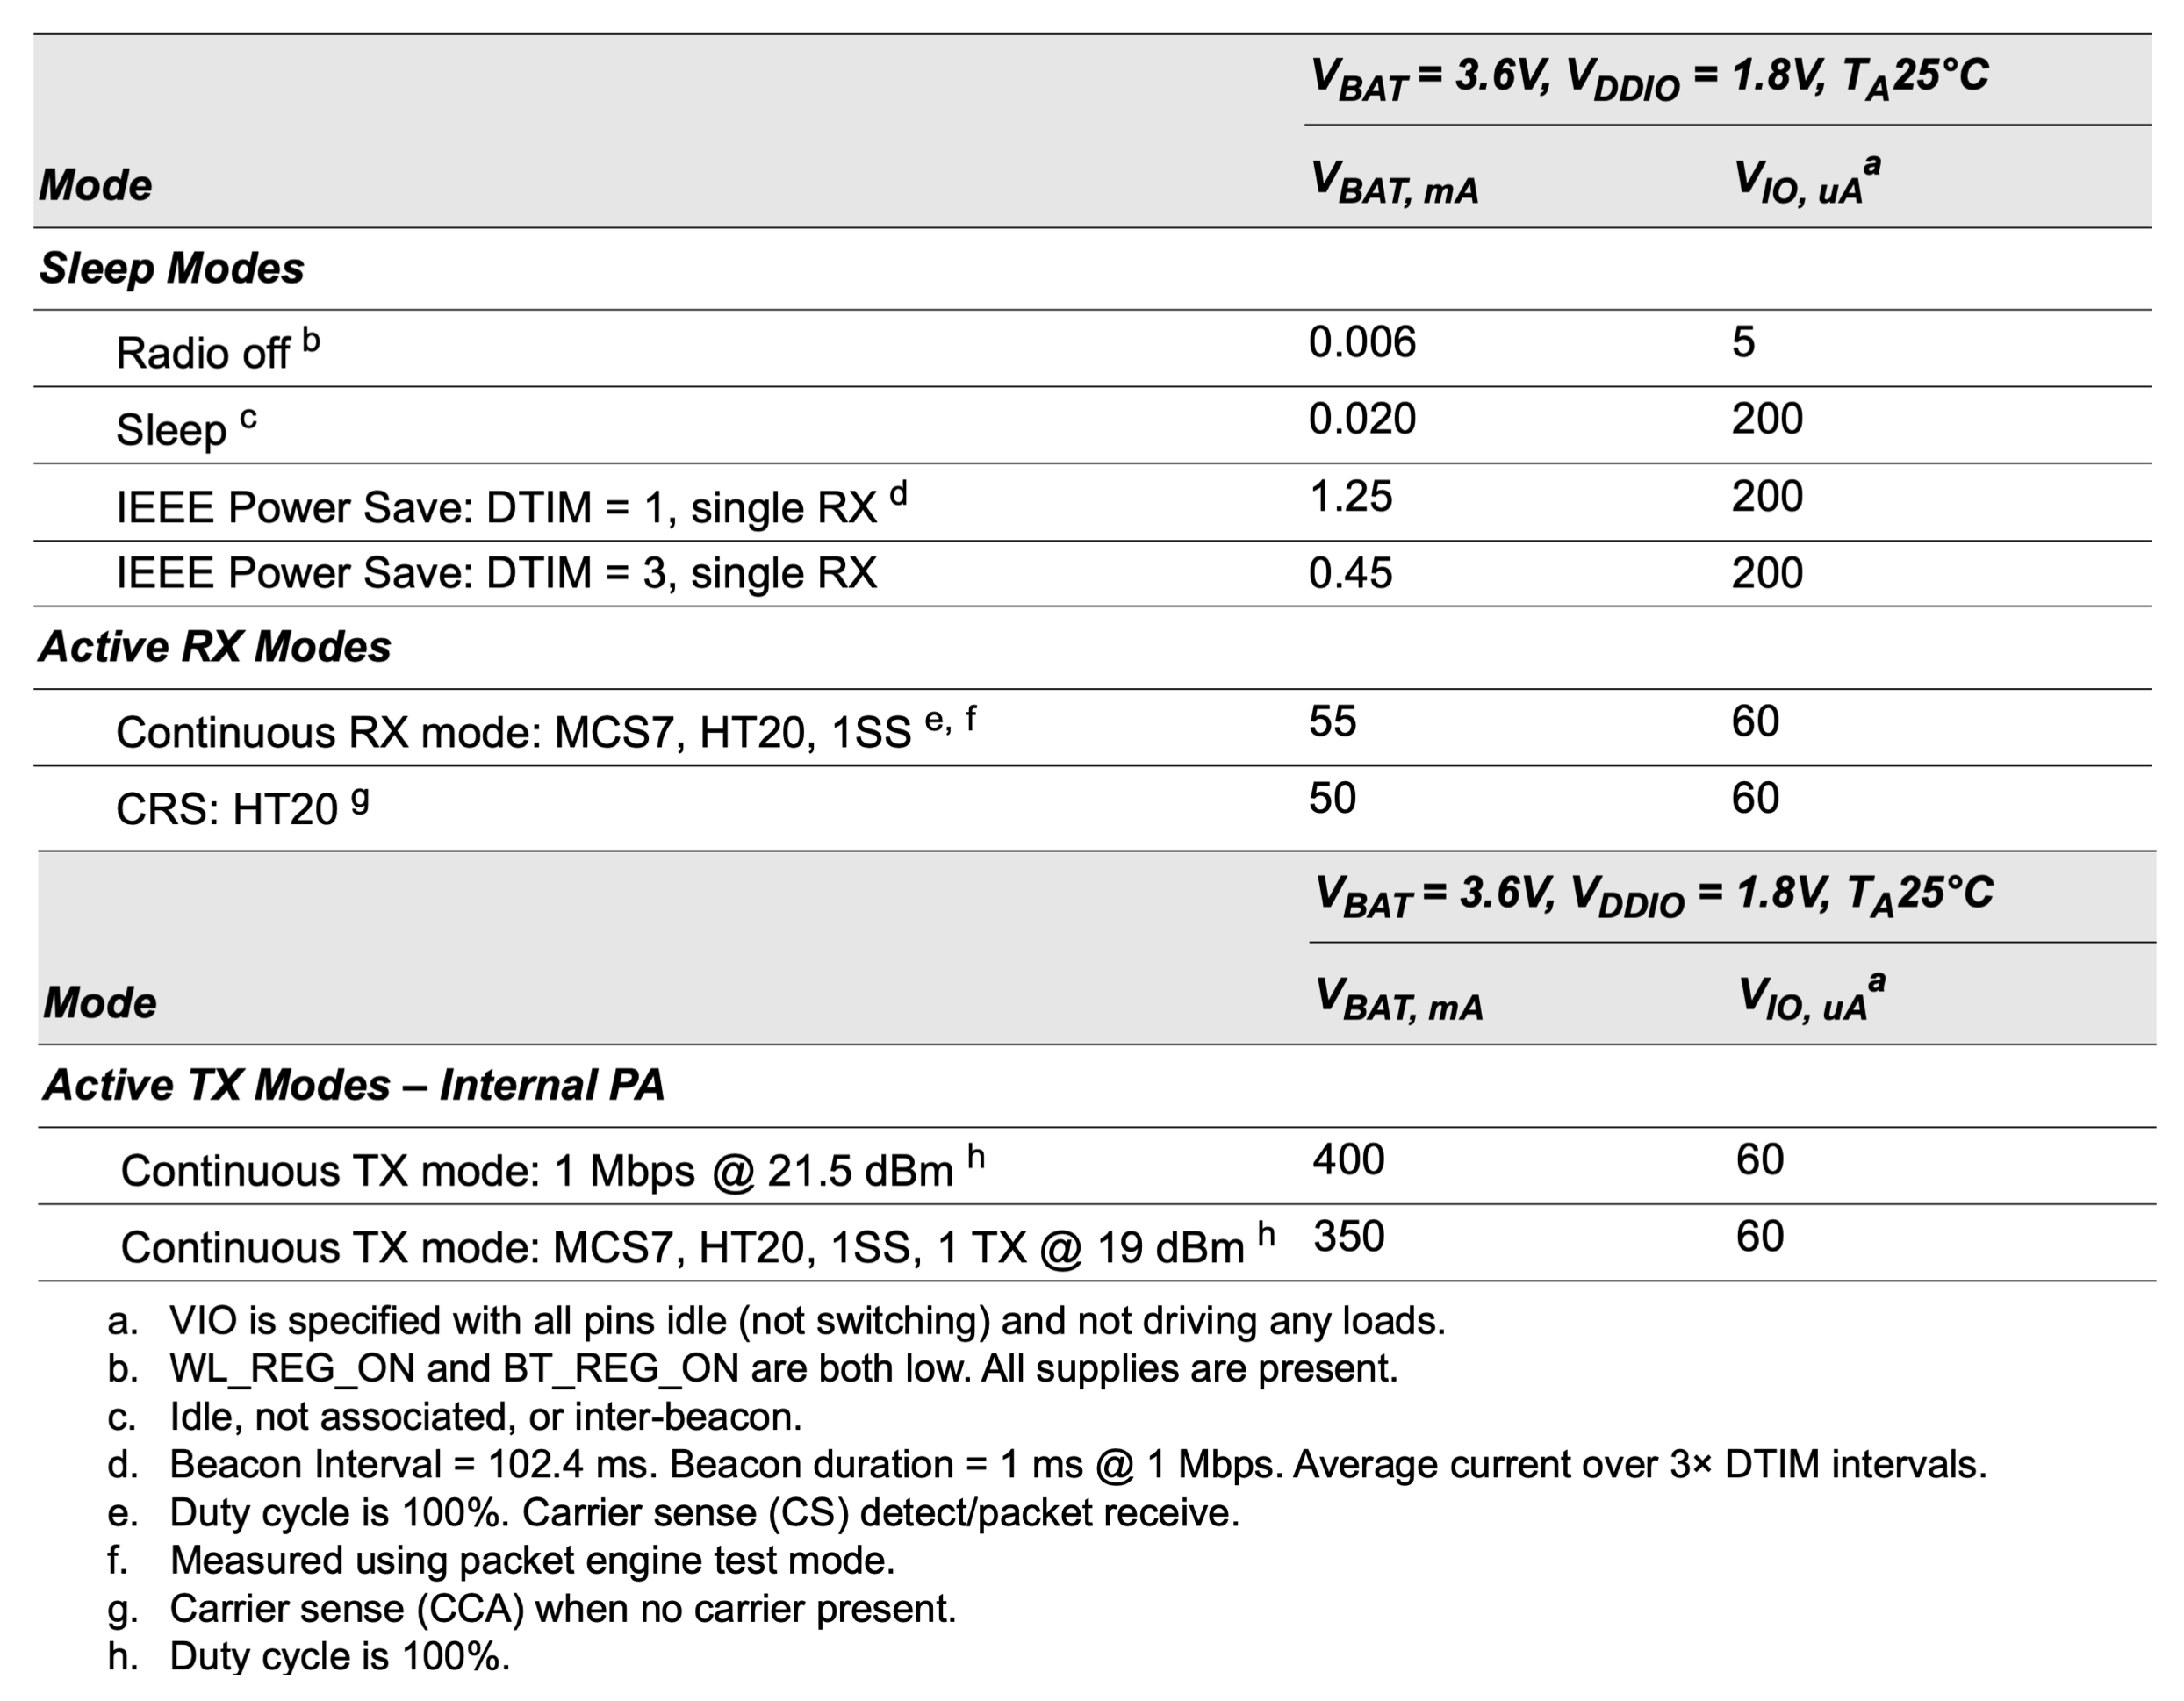
\includegraphics[scale=0.25]{Figs/datasheet.png}    
    \end{center}
    \caption{Current and Voltage values for BCM43455}
    \label{fig:bcm}
\end{figure}

Given this information, we can estimate the power \texttt{P} that the wifi adapter would use in this case when its 
turned on. Consider an app \texttt{A} which finishes executing in about \texttt{t} seconds. The total energy 
consumed (by the wifi adapter) by running \texttt{A} would then be calculated by \texttt{E = P * t}. \\
In order to calculate the estimated energy for specific block of code, such as ones which handle communication, all one 
needs to do is instrument the app to log execution time for that specific block of code. And then we can 
calculate the energy usage of that specific portion of program. The main idea behind this approach to 
estimate energy is that software developers don't usually have the technical equipment required to 
individually measure current and voltage values of actual devices. Given that setback, estimating energy 
consumption off of publicly available data sheets and runtime information from the app itself is a 
pretty reliable way to gather the required data. \\
\section{Calculating Optimal Chunk Size}
As mentioned before, our study focuses on optimizing communication cost of apps for IoT edge devices. 
Even though the best practices involved in this case do perform well for average case, our hypothesis 
is that after a communication pipe is established between the client and the server, having data sent or 
received in different chunk sizes could have an impact on the energy consumption of the whole process. 
The motivation behind this is that even though hardware optimizations such as power saving modes improve 
energy consumption efficiency, there are still software related configurations that can be altered to reduce 
the overall energy usage. We chose to focus on communication cost because it is an integral part of more or less 
every app deployed on an edge device where it communicated with the server one way or another to transmit 
some sort of data. \\
But why communication cost? Indeed, there are multiple code related factors that can help optimize energy 
consumption but our work is done under the assumption that these factors, such as data collection, via the 
sensor, the disk I/O operations etc. differ heavily from use-case to use-case and any alteration in code 
functionality to them, may affect their usage in real world. For example, a device monitoring a patient's 
heartbeat continuously is bound to use more energy than, let's say, monitoring every five minutes. 
However, in such critical examples, these types of optimizations severely undermine the actual 
functionality of the app. Therefore, our approach addresses a factor that is independent of the sensor 
usage in such a context and can potentially work on diverse examples. \\
To better explain how we calculate the optimal chunk size, we will first define energy-per-byte or EPB. 
It is a metric we use to determine which chunk size consumes the least amount of energy. \\

\begin{definition}
    \textbf{EPB} or Energy-per-Byte is defined as the amount of energy consumed when a single byte of data is sent from one device to another.
\end{definition}

But why is EPB an important factor rather than the overall energy consumed for the corresponding chunk size? 
We will explain this with the help of an example. Consider an app \texttt{C} on the edge device \texttt{EdgeD} that needs 
to send 256 bytes to the server-side app \texttt{S}. Assume you calculated the energy to send data at a 
chunk size of 64 bytes was the lowest at \texttt{E1} Joules. However, if you used 128 bytes at a time to 
send this data, you consume \texttt{E2} Joules which is slightly more than \texttt{E1}. In this case, 
we can not say the 64 bytes is the optimal chunk size for \texttt{EdgeD} because it would take \texttt{E1*4} 
amounts of energy to send the complete data and \texttt{E2*2} on the other hand. For the sake of this 
example, assume \texttt{E1} has the arbitrary value of 2 Joules (actual values are way way less and are usually 
in microJoules) and \texttt{E2} has the arbitrary value of 3 Joules. 64 bytes would take 8 Joules in total 
to send 256 bytes of data where as 128 bytes of chunk size would only use 6 Joules. That is why, EPB is an 
important factor and metric in this case. So what we need to do is divide \texttt{E1} by 64 and \texttt{E2} 
by 128 to get the EPB for their respective chunk sizes. Now, the lower energy consumption value of the 
two would be the optimal one as it would consume the lowest amount of energy among different chunk sizes. \\
To calculate the optimal chunk size on an edge device, we deploy a Python script which comprises of a 
list of different chunk sizes of order \texttt{$2^{n}$} where \texttt{n} by default can be anything between 
1 and 30 (included). The upper limit can be adjusted depending on the use case of the program. It then 
proceeds to send data in different chunk sizes and then measure the time it took for the communication to take 
place. This time is then used to calculated the overall energy consumption for sending a specific amount of 
data. \\
This is a pretty straightforward but novel approach to aid programmers in developing applications for 
a target edge device where they can optimize the communication cost in terms of energy. In some use cases, the 
difference is considerable while in others it may not be that much. In short, it depends on the nature of the app 
itself. The following section will clarify more as to why it is as we describe our experimental and nature of the 
apps, and discuss our results. \\